% Chapter Electrodes

\chapter{Electrodes Design with Electrostatic Simulation} % Main chapter title

\label{ChapterElectrodes} % Change X to a consecutive number; for referencing this chapter elsewhere, use \ref{ChapterX}

%----------------------------------------------------------------------------------------
%	BEGING CHAPTER
%----------------------------------------------------------------------------------------

Let me tell you about my work with an electrostatic simulation software called COMSOL.
That was quite nice. Just designing the detector and the aluminium electrodes with a beautiful and efficient interface.
Thanks to that, I could simulate a lot of configuration and geometry to probe for the finest results out there.
Finest meaning a lot of fiducial volume, good charge collection, and low electric capacity.
A usual impossible to solve problem which lead to a lot of trade-off in itself, without adding the issues about the heat channel.
But hey, I could obtain some nice plots and tables, check them out.


\section{Crosstalk}

Yep, goota talk about the link between the crosstalk on the ionization channels and the capacitance term between those electrodes.
We can simply say for now that the higher the capacitance is and the higher the crosstalk will be. However, it should be very interesting to quantify the link between these two quantities.
Linking the crosstalk matrix and the capacitance matrix, and be able to compare that experimentally.

\section{Appendix: Detectors fields lines}

\begin{figure}
\centering
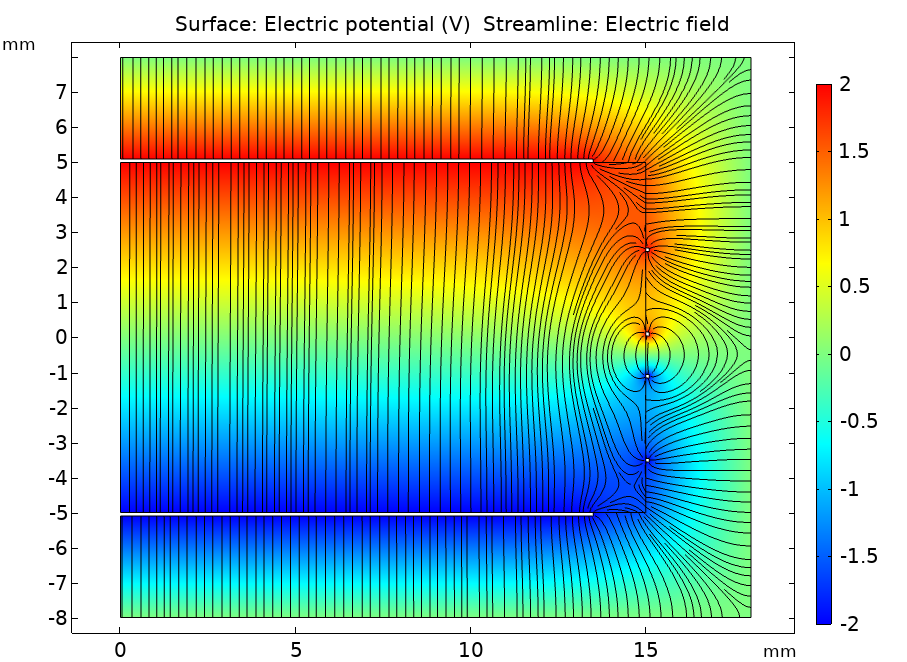
\includegraphics[width=\linewidth]{Figures/Electrodes/streamlines_red80.png}
\caption{Streamlines of the electric field in RED80.}
\label{fig:streamlines-red80}
\end{figure}
